%%%%%%%%%%%%%%%%%%%%%%%%%%%%%%%%
% Settings
%%%%%%%%%%%%%%%%%%%%%%%%%%%%%%%%

\newif\ifbatchgrad
\newif\ifsecondorder

\batchgradtrue
\batchgradfalse
\secondordertrue
\secondorderfalse

\usetikzlibrary{arrows.meta}




%%%%%%%%%%%%%%%%%%%%%%%%%%%%%%%%%%

\newif\ifanyextension
\anyextensionfalse
\ifsecondorder
	\anyextensiontrue
\fi
\ifbatchgrad
	\anyextensiontrue
\fi

\colorlet{newMessageFill}{white}
\colorlet{newMessageDraw}{red}
\colorlet{messageFill}{white}
\colorlet{messageDraw}{black}
\colorlet{moduleFrame}{black!80!white}
\colorlet{moduleFill}{black!30!white}
\colorlet{moduleContentFill}{black!10!white}


\tikzset{thickArrow/.style={
		%->,
		-{Latex[length=1mm,width=2mm]},
		thick,
		rounded corners=1ex
	}
}
\tikzset{newThickArrow/.style={
		thickArrow,
		very thick,
		rounded corners=1ex,
		newMessageDraw,
	}
}

\tikzset{module/.style={
		rounded corners=1ex,
		draw=moduleFrame,
		fill=moduleFill,
		inner sep=0
	}
}
\tikzset{moduleContent/.style={
		rounded corners=1ex,
		draw=moduleFrame,
		fill=moduleContentFill,
		inner sep=0
	}
}

\tikzset{message/.style={
		rectangle,
		rounded corners=1ex,
		minimum width=19ex,
		minimum height=3.5ex,
		draw=messageDraw,
		fill=messageFill
	}
}
\tikzset{newMessage/.style={
		rectangle,
		rounded corners=1ex,
		minimum width=19ex,
		minimum height=3.5ex,
		thick,
		draw=newMessageDraw,
		fill=newMessageFill
	}
}


\newcommand{\va}{\bm{a}}
\newcommand{\vb}{\bm{b}}
\newcommand{\vtheta}{\bm{\theta}}
\newcommand{\jac}{\mathrm{J}}
\newcommand{\mS}{\bm{S}}

%%%%%%%%%%%%%%%%%%%%%%%%%%%%%%%%
% Actual plotting
%%%%%%%%%%%%%%%%%%%%%%%%%%%%%%%%

\small
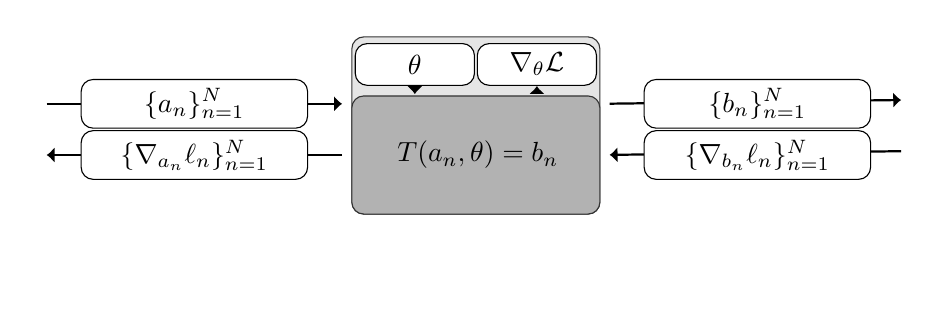
\begin{tikzpicture}
\node (v1) at (0.65,0.6) {};
\node (v2) at (-2.5,2.85) {};
\node (v3) at (-2.5,2.1) {};
\node (vother) at (0.65,-0.25) {};

\draw[moduleContent] (v2) rectangle (v1);

\ifanyextension
\draw[moduleContent] (v3) rectangle (vother);
\fi

\draw[module] (v3) rectangle (v1) {};

\node (v16) at (-1.7,2.6) {};
\node (v17) at (-1.7,2) {};
\draw[thickArrow] (v16) edge (v17);

\node (v4) at (4.6,2.05) {};
\node (v6) at (4.6,1.4) {};
\node (v8) at (4.6,0.75) {};
\node (v5) at (0.65,2) {};
\node (v7) at (0.65,1.35) {};
\node (v9) at (0.65,0.7) {};
\draw[thickArrow] (v5) edge (v4);
\draw[thickArrow] (v6) edge (v7);
\node (v10) at (-2.5,2) {};
\node (v12) at (-2.5,1.35) {};
\node (v14) at (-2.5,0.7) {};
\node (v11) at (-6.5,2) {};
\node (v13) at (-6.5,1.35) {};
\node (v15) at (-6.5,0.7) {};
\draw[thickArrow] (v11) edge (v10);
\draw[thickArrow]  (v12) edge (v13);

\node at (-0.9,1.35) {$T(\va_n, \vtheta) = \vb_n$};

\node[message] at (-4.5,2) {$\{\va_n\}_{n=1}^N$};
\node[message] at (2.65,2) {$\{\vb_n\}_{n=1}^N$};
\node[message] at (-4.5,1.35) {$\{\nabla_{\va_n} \ell_n\}_{n=1}^N$};
\node[message] at (2.65,1.35) {$\{\nabla_{\vb_n} \ell_n\}_{n=1}^N$};



\ifbatchgrad
\node[newMessage] at (-0.9,0.1) {$\{\nabla_{\vtheta} \ell_n\}_{n=1}^N$};
\fi

\ifsecondorder
\draw[newThickArrow] (v14) edge (v15);
\draw[newThickArrow] (v8) edge (v9);
\node[newMessage] at (2.65,0.7) {$\{[\jac_{\vb_n} f_n]^\top\mS_n\}_{n=1}^N$};
\node[newMessage] at (-4.5,0.7) {$\{[\jac_{\va_n} f_n]^\top\mS_n\}_{n=1}^N$};
\node[newMessage] at (-0.9,0.15) {$\{[\jac_{\vtheta} f_n]^\top \mS_n\}_{n=1}^N$};
\fi

\ifanyextension
\node (v20) at (-0.9,0.7) {};
\node (v21) at (-0.9,0.35) {};
\draw[newThickArrow] (v20) edge[out=-90,in=90] (v21);
\fi


\node[message,minimum width=10ex] at (-1.7,2.5) {$\vtheta$};
\node[message,minimum width=10ex] at (-0.15,2.5) {$\nabla_{\vtheta} \mathcal{L}$};

\node (v18) at (-0.15,2) {};
\node (v19) at (-0.15,2.35) {};
\draw[thickArrow] (v18) edge (v19);

\end{tikzpicture}